\section{Concept development}

...\newpage

\section{Project structure}

...\newpage

\section{Simple mathematical computation examples for Parallel Programming}

As a first example, which we try to implement on our ESP32, we will discuss a similar computation as already mentioned in Chapter \ref{chap:mathComp}. In formula \ref{formula:scalarProdSeq}, we have pointed out that the computation of a simple scalar product of two vectors with the same dimension \textit{N} can be split into several sub task \textit{p}. Our modified version is based on two sums. The outer one will iterate [index \textit{i}, see formula \ref{formula:twoLoopSum}] from zero to an upper limit \textit{N\textsubscript{1}} and sum up the result from the inner sum, which will perform a sum from 0 to \textit{N\textsubscript{2}} [index \textit{j}, see formula \ref{formula:twoLoopSum}] over a multiplication of \textit{i} and \textit{j}. The following formula represent the announced mathematical problem:

\begin{align} \label{formula:twoLoopSum}
	\begin{aligned}
	s &= \sum_{i = 0}^{i} \left( \sum_{j = 0}^{j} \left(i \cdot j\right) \right)
	\end{aligned}
\end{align}
\

To process the problem in parallel, it is only possible to seperate the outer sum into sub sums regarding to formula \ref{formula:twoLoopSumParallel}.

\begin{align} \label{formula:twoLoopSumParallel}
	\begin{aligned}
	s &= \sum_{i = 0}^{N_1} \left( \sum_{j = 0}^{N_2} \left(i \cdot j\right) \right)
	\\ &=  \underbrace{ 
			\sum_{i = 0}^{\frac{N_1}{2} - 1} \left( \sum_{j = 0}^{N_2} \left(i \cdot j\right) \right)
 		}_\text{p\textsubscript{0}} \qquad \vertarrowbox{+}{process communication} \qquad \underbrace{  
 			\sum_{i = \frac{N_1}{2}}^{N_1} \left( \sum_{j = 0}^{N_2} \left(i \cdot j\right) \right)
		}_\text{p\textsubscript{1}}
	\end{aligned}
\end{align}
\

For collecting the part results from the parallel computed sums, some sort of process communication between the threads is necessary, more then, its impossible without it. But actually, this is the task, we have to take care about most. Otherwise we will run into race conditions while addressing same resources or even blocking methods, which will result in wrong execution time measurements.

\newpage

\subsection{UML diagram}

\begin{figure}[htbp]
	\centerline{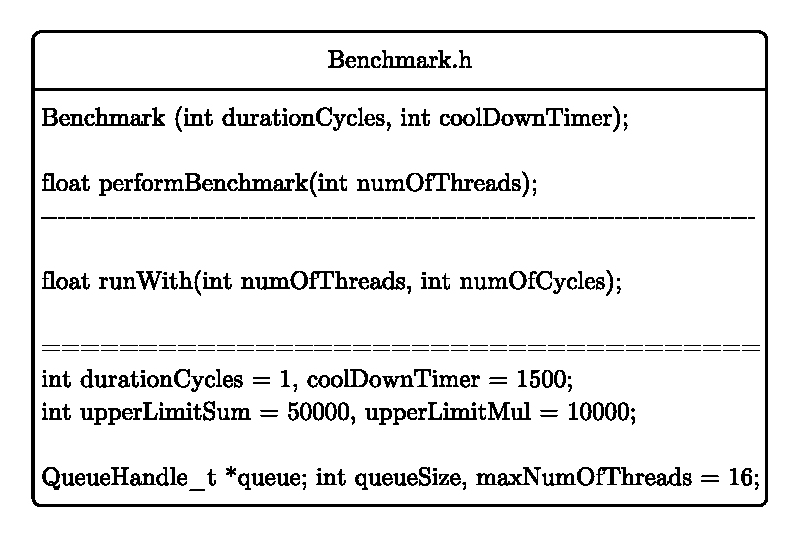
\includegraphics[width=.6\linewidth]{images/Benchmark-UML.pdf}}
	\caption{ UML class diagram of the Benchmark object }
	\label{fig:benchUML}
\end{figure}

\begin{figure}[htbp]
	\centerline{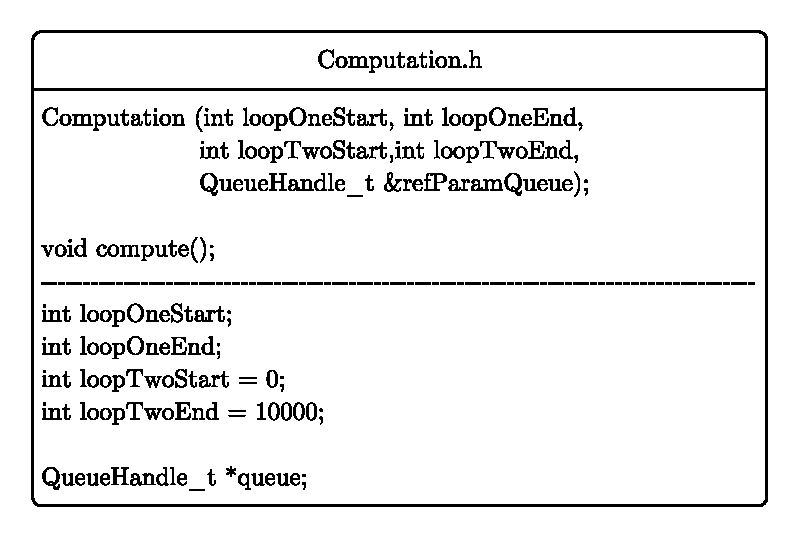
\includegraphics[width=.6\linewidth]{images/Computation-UML.pdf}}
	\caption{ UML class diagram of the Computation object }
	\label{fig:compUML}
\end{figure}

\newpage

\section{Class diagramm}

...

\subsection{C++ Backend benchmark}

...

\subsection{Vuejs Frontend}

...\newpage

\section{Benchmark setup}

...
